\section*{Problem 1}

Draw $|Xs(\omega)|$ for the following cases if $x_s(t)=x(t)p(t)$ with sampling period T.

\begin{equation*}
p(t) = \displaystyle\sum_{n=-\infty}^{n=\infty} \delta(t-nT).
\end{equation*} 

\begin{figure}[H]
\caption*{}
\centering
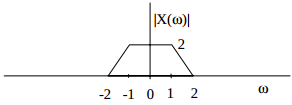
\includegraphics[width=0.4\textwidth]{figs/c3p11.png}
\label{fig:c3p11}
\end{figure} 

\subsection*{Solution}

The minimum sampling period of the signal according to the Nyquist theorem is:

\begin{equation*}
\begin{aligned}
\omega_m &= 2 \\
\omega_{Ns} >&= 2 \omega_m >= 4 \\
T_{Ns} &= \frac{2 \pi}{\omega_s} <= \frac{\pi}{2}
\end{aligned}
\end{equation*} 

\begin{itemize}
\item $T_s = \pi/4 sec$
\end{itemize} 

This sampling period is lower than the minimum required and therefore no
aliasing will occur as can be seen in (\ref{fig:c3p1a}).

\begin{equation*}
\omega_s = \frac{2 \pi}{T_s} = 8 
\end{equation*} 

\zcodemat{sources/c3p1a.m}{Plot of $|X_s(\omega)|$}

\begin{figure}[H]
\caption{Sampling $|X_s(\omega)|$}
\centering
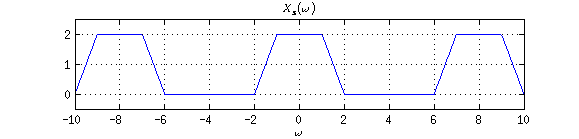
\includegraphics[width=0.6\textwidth]{figs/c3p1a.png}
\label{fig:c3p1a}
\end{figure}

\begin{itemize}
\item $T_s = \pi/2 sec$
\end{itemize} 

This sampling period is equal than the minimum required and therefore is
in the limit of no aliasing as can be seen in (\ref{fig:c3p1b}).

\begin{equation*}
\omega_s = \frac{2 \pi}{T_s} = 4
\end{equation*} 

\begin{figure}[H]
\caption{Sampling $|X_s(\omega)|$}
\centering
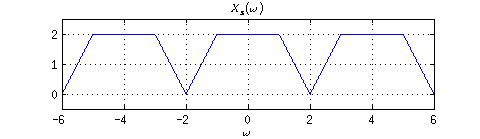
\includegraphics[width=0.6\textwidth]{figs/c3p1b.png}
\label{fig:c3p1b}
\end{figure}

\begin{itemize}
\item $T_s = 2 \pi/3 sec$
\end{itemize} 

This sampling period is lower than the minimum required and therefore 
aliasing will occur as can be seen in (\ref{fig:c3p1c}).

\begin{equation*}
\omega_s = \frac{2 \pi}{T_s} = 4
\end{equation*} 

\begin{figure}[H]
\caption{Sampling $|X_s(\omega)|$}
\centering
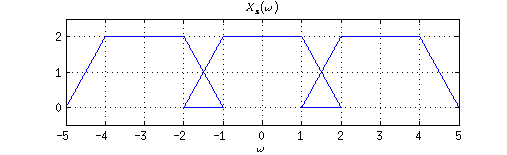
\includegraphics[width=0.6\textwidth]{figs/c3p1c.png}
\label{fig:c3p1c}
\end{figure}



